%\documentclass[a4paper,10pt]{article}
\documentclass[10pt]{article}
\usepackage[utf8]{inputenc}
\usepackage{xspace}
\usepackage{url}
\usepackage{graphicx,graphics} 
\usepackage{color}
\usepackage{amsmath}
\usepackage{amsfonts}
\usepackage{amssymb}
\usepackage{amsthm}
\usepackage{algorithm}
\usepackage{algorithmic}
\usepackage{longtable}
\usepackage{complexity}
\usepackage{tkz-graph}
\usepackage{float}
\usepackage{tabularx}
\usepackage{setspace}
\usepackage{icomma}
\renewcommand{\algorithmicrequire}{\textbf{Input:}}
\renewcommand{\algorithmicensure}{\textbf{Output:}}
\usepackage{authblk}
\usepackage[colorlinks=true,breaklinks=true,linkcolor=blue]{hyperref}


\newcommand\rmatching{${\cal R}$-matching\xspace}
\newcommand\mdelay{$\cal M$-delay\xspace}
\newcommand\matchedgraph{{\bf matched graph}}
\newtheorem{proposition}{Proposition}
\newtheorem{theorem}{Theorem}

\setlength{\parskip}{1ex} % Espace entre les paragraphes

\newtheorem{fact}{Fact}
\newtheorem{lemma}[theorem]{Lemma}
\newtheorem{definition}{Definition}
\newtheorem{corollary}{Corollary}

% \renewcommand{\thefootnote}{\*}

\newcommand{\todo}[1]{{\color{red} TODO: {#1}}}
\newcommand\pazl{\textsc{pazl}\xspace}
\newcommand\pall{\textsc{pall}\xspace}
\newcommand\bra{\textsc{bra}\xspace}
\newcommand\pra{\textsc{pra}\xspace}
\newcommand\minpra{\textsc{min-pra}\xspace}
%opening
\title{Deterministic Scheduling of Periodic Messages for Cloud RAN}
 

\author[1]{Dominique Barth}
\author[1,2]{Ma\"el Guiraud}
% \author[1]{Christian Cad\'er\'e}
 \author[2]{Brice Leclerc}
 \author[2]{Olivier Marc\'e}
\author[1]{Yann Strozecki}
\affil[1]{David Laboratory, UVSQ}
\affil[2]{Nokia Bell Labs France}

\begin{document}

\maketitle\section{Model and Problems}\label{sec:def}

We use the notation $[n]$ to denote the interval of $n$ integers $\{0,\dots,n-1\}$.


  \subsection{Network modeling}
  
The network is modeled as a directed graph $G=(V,A)$. Each arc  $(u,v)$ in $A$ is labeled by an integer weight $\Omega(u,v)$ which represents the time taken by a message to go from $u$ to $v$ using this arc. A {\bf route} $r$ in $G$ is a directed path, that is, a sequence of adjacent vertices $u_0, \ldots , u_{l}$, with $(u_i,u_{i+1}) \in A$.  The {\bf delay} of a vertex $u_i$ in a path $r=(u_0,\dots,u_l)$ is defined by $\lambda(u_i,r)= \sum\limits_{0 \leq j <i} \Omega(u_j, u_{j+1})$. We also define $\lambda(u_0,r)=0$. The length of the route $r$ is defined by $\lambda (r)= \lambda (u_l,r)$.
We denote by $\cal R$ a set of routes, the pair $(G,\cal R)$ is called a {\bf routed network} and represents our telecommunication network.
The first vertex of a route models an antenna (RRH) and the last one a data-center (BBU) which computes the messages sent by the antenna.

   \subsection{Messages dynamic}
	 
    Time is discretized, hence the unit of all time values is a {\bf tic}, the time needed to transmit a minimal unit of data over the network. The weight of an arc is also expressed in tics, it is the time needed by a message to go through this arc.
        In the process we study, a {\bf frame} is sent on each route at each period, denoted by $P$.
        A frame $F$ is composed of several {\bf datagrams}. The size of a frame, denoted $|F|$ is the number of datagrams in the frame. The datagrams $\{d_0,\ldots,d_{|F|}\}$ of a frame represent one or several \emph{consecutive tics}, called length of the datagram. Once a datagram have been emitted, it can not be severed during its travel in the network. Thus, the length of a frame is $\sum_{i=0}^{{|F|}} d_i = \tau$. In this paper, we assume that $\tau$ is the same for all routes. Indeed, the data flow sent by an RRH to its BBU is the same, regardless of the route.
        
      Let $r=(u_0,\dots,u_l)$ be a route, a datagram $d_j$ of lenght $|d_j|$ can be buffered in a node $u_i$, during at least $|d_j|$ tics. A datagram $d_j$ is thus characterized by a sequence $\{b_j^0,\ldots,b_j^l\}$ of buffers corresponding to the buffering time of this datagram in a node $ u_i$. We denote by $m_r(d_j)$ the time at which a datagram $d_j$ is sent at time from $u_0$ the first vertex of $r$ then it will arrive at vertex $u_i$ in $r$ at time $m_r(d_j) + \lambda(u_i,r) + \sum_{k=0}^{i-1}b_j^k$. Since the process is periodic, if the datagram from $r$ goes through an arc at time $t\in [0,P-1]$,  then it goes through the same arc at time $t+kP$ for all positive integers $k$. Therefore, every time value can be computed modulo $P$ and we say that the first time slot at which a datagram $d_j$ sent at time $m_r(d_j)$ on $r$ reaches a vertex $u_i$ in $r$ is $t(d_j,u_i,r) = m_r(d_j) + \lambda(u_i,r) + \sum_{k=0}^{i-1}b_j^k \mod P$. 
      
      A frame is thus defined as follow on the route $i$ : $$F_i = \{ (m_i(d_0),\{b_0^{0,i},\ldots,b_0^{l,i}\}),\ldots,(m_i(d_{|F_i|}),\{b_{|F_i|}^{0,i},\ldots,b_{|F_i|}^{l,i}\}) \}$$, where $|F|$ is the number of datagrams in the frame, and $l$ the number of nodes in the routes.
      
       Let us call $[t(F,u,r)]_{P,\tau}$ the set of time slots used by a frame $F$ on a route $r$ at vertex $u$ in a period $P$, that is $[t(F,u,r)]_{P,\tau} = \{t(d_0,u,r) + i \mod P \mid 0 \leq i < |d_0|\} \cup \ldots \cup \{ t(d_{|F|},u,r) + i \mod P \mid 0 \leq i < |d_{|F|}|\}  $.
%       Usually $P$ and $\tau$ will be clear from the context and we will denote $[t(v,r)]_{P,\tau}$ by $[t(v,r)]$.
      Let $r_1$ and $r_2$ be two routes, on which frames $F_1$ and $F_2$ are sent in their first vertex.
      We say that the two routes have a {\bf collision} if they share an arc $(u,v)$ and $[t(F_1,u,r_{1})]_{P,\tau} \cap [t(F_2,u,r_{2})]_{P,\tau} \neq \emptyset$.
      
         A {\bf $(P,\tau)$-periodic assignment} of a routed network $(G,\cal R)$ is a function that associates to each datagram of each frame of each route 
         $r \in \cal R$ its \textbf{offset} $m_r(d_i)$ that is the time at which the datagram $d_i$ is emitted at the first vertex of the route $r$ and its buffers $\{b_i^{0,r},\ldots,b_i^{l,r}\}$ that is, the buffering time of the datagram in each nodes of the routes. In a $(P,\tau)$-periodic assignment, \emph{no pair of routes has a collision}.
	 
	 
%      As an example of a $(2,1)$-periodic assignment, let us consider a routed network 
%      where all pairs of routes intersect at a different arc. It is easy to design such a network and an example is given in Figure~\ref{fig:example}. We set $\tau = 1$, thus each frames have only one datagram of size $1$, and the weights are chosen so that if $r_{i}$ and $r_{j}$ have $u$ as first common vertex then we have $\lambda(u,r_{i}) - \lambda(u,r_{j})=1$. There is a $(2,1)$-periodic assignment by setting all $m_{i}(d)$ to $0$.
%
%  
%      \begin{figure}[ht]
%      \begin{center}
%          \scalebox{0.47}{
%          
%\begin{tikzpicture}
%
%
%\tikzset{
%  LabelStyle/.style = { rectangle, rounded corners, draw,
%                       font = \bfseries },
%  EdgeStyle/.append style = {->} }
%  \SetGraphUnit{5}
%  \node[draw,circle] (s3) at (4, 2) {$s_2$}; 
%  \node[draw,circle] (s2) at (0, 4) {$s_1$}; 
%  \node[draw,circle] (s1) at (0, 6) {$s_0$}; 
%
%  \node[draw,circle] (t3) at (14, 7) {$t_2$}; 
%  \node[draw,circle] (t2) at (14, 4) {$t_1$}; 
%  \node[draw,circle] (t1) at (10, 2) {$t_0$}; 
%
%  
%  \SetVertexNoLabel
%  \Vertex[x=2,y=5]{A}
%  \Vertex[x=4,y=5]{B}
%  \Vertex[x=10,y=5]{C}
%  \Vertex[x=12,y=5]{D}
%  \Vertex[x=6,y=3]{E}
%  \Vertex[x=8,y=3]{F}
%  \tikzset{
%  EdgeStyle/.append style = {green} }
%  \Edge[label = 2](s2)(A)
%  \Edge[label = 1](A)(B)
%  \Edge[label = 2](B)(C)
%  \Edge[label = 1](C)(D)
%  \Edge[label = 1](D)(t2)
%
%  
%   \tikzset{
%  EdgeStyle/.append style = {red} }
%  \Edge[label = 2](s3)(E)
%  \Edge[label = 1](E)(F)
%  \Edge[label = 1](F)(C)
%  \Edge[label = 1](C)(D)
%  \Edge[label = 1](D)(t3) 
%     \tikzset{
%  EdgeStyle/.append style = {blue} }
%  \Edge[label = 1](s1)(A)
%  \Edge[label = 1](A)(B)
%  \Edge[label = 1](B)(E)
%  \Edge[label = 1](E)(F)
%  \Edge[label = 1](F)(t1)
%
%\end{tikzpicture}
%
%}
%     \end{center}
%       \caption{A routed network with $(0,0,0)$ as a $(2,1)$-periodic assignment}
%       \label{fig:example}
%      \end{figure}

      \subsection{Periodic route assignment}\label{nonmonotone}

    We want to find an assignment which allows to send periodic messages from sources to targets
    without collisions. We introduce the following associated decision problem, useful for hardness proofs.
    

      \noindent {\bf  Periodic Routes Assignment (\pra)} 

      \noindent {\bf Input:} a routed network $(G,\cal R)$, an integer $\tau$ and an integer $P$, a set of frames ${\cal F}$

      \noindent {\bf Question:} does there exist a $(P,\tau)$-periodic assignment of $(G,\cal R)$ ?

%
%      We will prove in Section~\ref{sec:complexity} that the problem \pra is $\NP$-complete, even in restricted settings.
%      In fact, approximating the smallest value of $P$ for which there is a $(P,\tau)$-periodic assignment is already hard.
%      
%      An unusual property of assignment is that given a routed network, we may have a $(P,\tau)$-periodic assignment but no
%      $(P',\tau)$-periodic assignment with $P' > P$: the existence of an assignment is not monotone with regard to $P$.
%
%	\begin{lemma} \label{lemma:monotonic}
%	 For any odd $P$, there is a routed network such that there is a $(2,1)$-periodic assignment but no $(P,1)$-periodic assignment.
%	\end{lemma}
%\begin{proof}
%
%      We consider a generalization of the routed network $(G,{\cal R})$ given in Figure~\ref{fig:example}. 
%      There are $n$ routes in the routed network and each pair of routes $(r_i,r_j)$ share a single arc, which is not in any other route. The weights are chosen so that for $v$, the first vertex which belongs to $r_i$ and $r_j$, we have $\lambda(v,r_i) - \lambda(v,r_j)= P$, where $P$ is an odd number smaller than $n$. In such a graph, there is no $(P,\tau)$-periodic assignment, since the problem reduces to finding a $P$-coloring in a complete graph with $n > P$ vertices, the colors being the offsets of the routes.\\
%      If we consider a period of $2$, for all $i \neq j$, $\lambda(v,r_i) - \lambda(v,r_j) \mod 2 = 1$ . Therefore $(0,\dots,0)$ is a $(2,1)$-periodic assignment of ${\cal R}$.      
%\end{proof}
      
      
      \subsection{Periodic assignment for low latency}
      
   In the context of cloud-RAN applications, we need to send a frame from an RRH $u$ to a BBU $v$ and then 
      we must send the answer from $v$ back to $u$. We say that a routed network $(G, {\cal R})$ is \textbf{symmetric} if the set of routes is partitioned into the sets $Fr$ of \textbf{forward routes} and $Br$ of \textbf{backward routes}. There is a bijection $\rho$ between $A$ and $B$ such that for any forward route $r \in A$ with first vertex $u$ and last vertex $v$, the backward route $\rho(r) \in B$ has first vertex $v$ and last vertex $u$. In all practical cases the routes $r$ and $\rho(r)$ will be the same with the orientation of the arcs reversed, which corresponds to bidirectional links in \emph{full-duplex} networks, but we need not to enforce this property.
         
      We now give a new interpretation of a $(P,\tau)$-periodic assignment of a $(G,{\cal R})$ symmetric routed network, so that it represents the sending of a frame and of its answer.
      This assignment represents the following process: First, the datagrams of a frame $F_r$ is sent at $u$, through the route $r \in A$, at time $\{m_r(d_0),\ldots,m_r(d_{|F_r|}) \}$.
      Those datagrams are received by $v$, i.e., the last vertex of $r$ at times $\{t(d_0,v,r),\ldots,t(d_{|F_r|},v,r)\}$. 
     Once $v$ has received all the datagrams of a frame, the answer is computed and sent back in a frame $F'_r$. Note that $|F'_r|$ may not be equal to $|F_r|$, i.e. the answer is not necessarily under the same form as the initial frame. Thus the node $v$ send $F'_r$ to  $u$ on the route $\rho(r)$.
      % in the same period at times $m_{\rho(r)}$ if $m_{\rho(r)} > t(v,r)$, otherwise at time $m_{\rho(r)}$ in the next period. 
      The time between the arrival of the last datagram of a frame and the time the answer is sent back is called the \textbf{waiting time} and is defined by $w_r$% = m_{\rho(r)} - t(v,r)$ if $m_{\rho(r)} > t(v,r)$ and $w_r = m_{\rho(r)} + P - t(v,r)$ otherwise. Figure~\ref{fig:assignment} illustrates this process in an RRH and its corresponding BBU.
 
     \begin{figure}[h]
      \begin{center}
      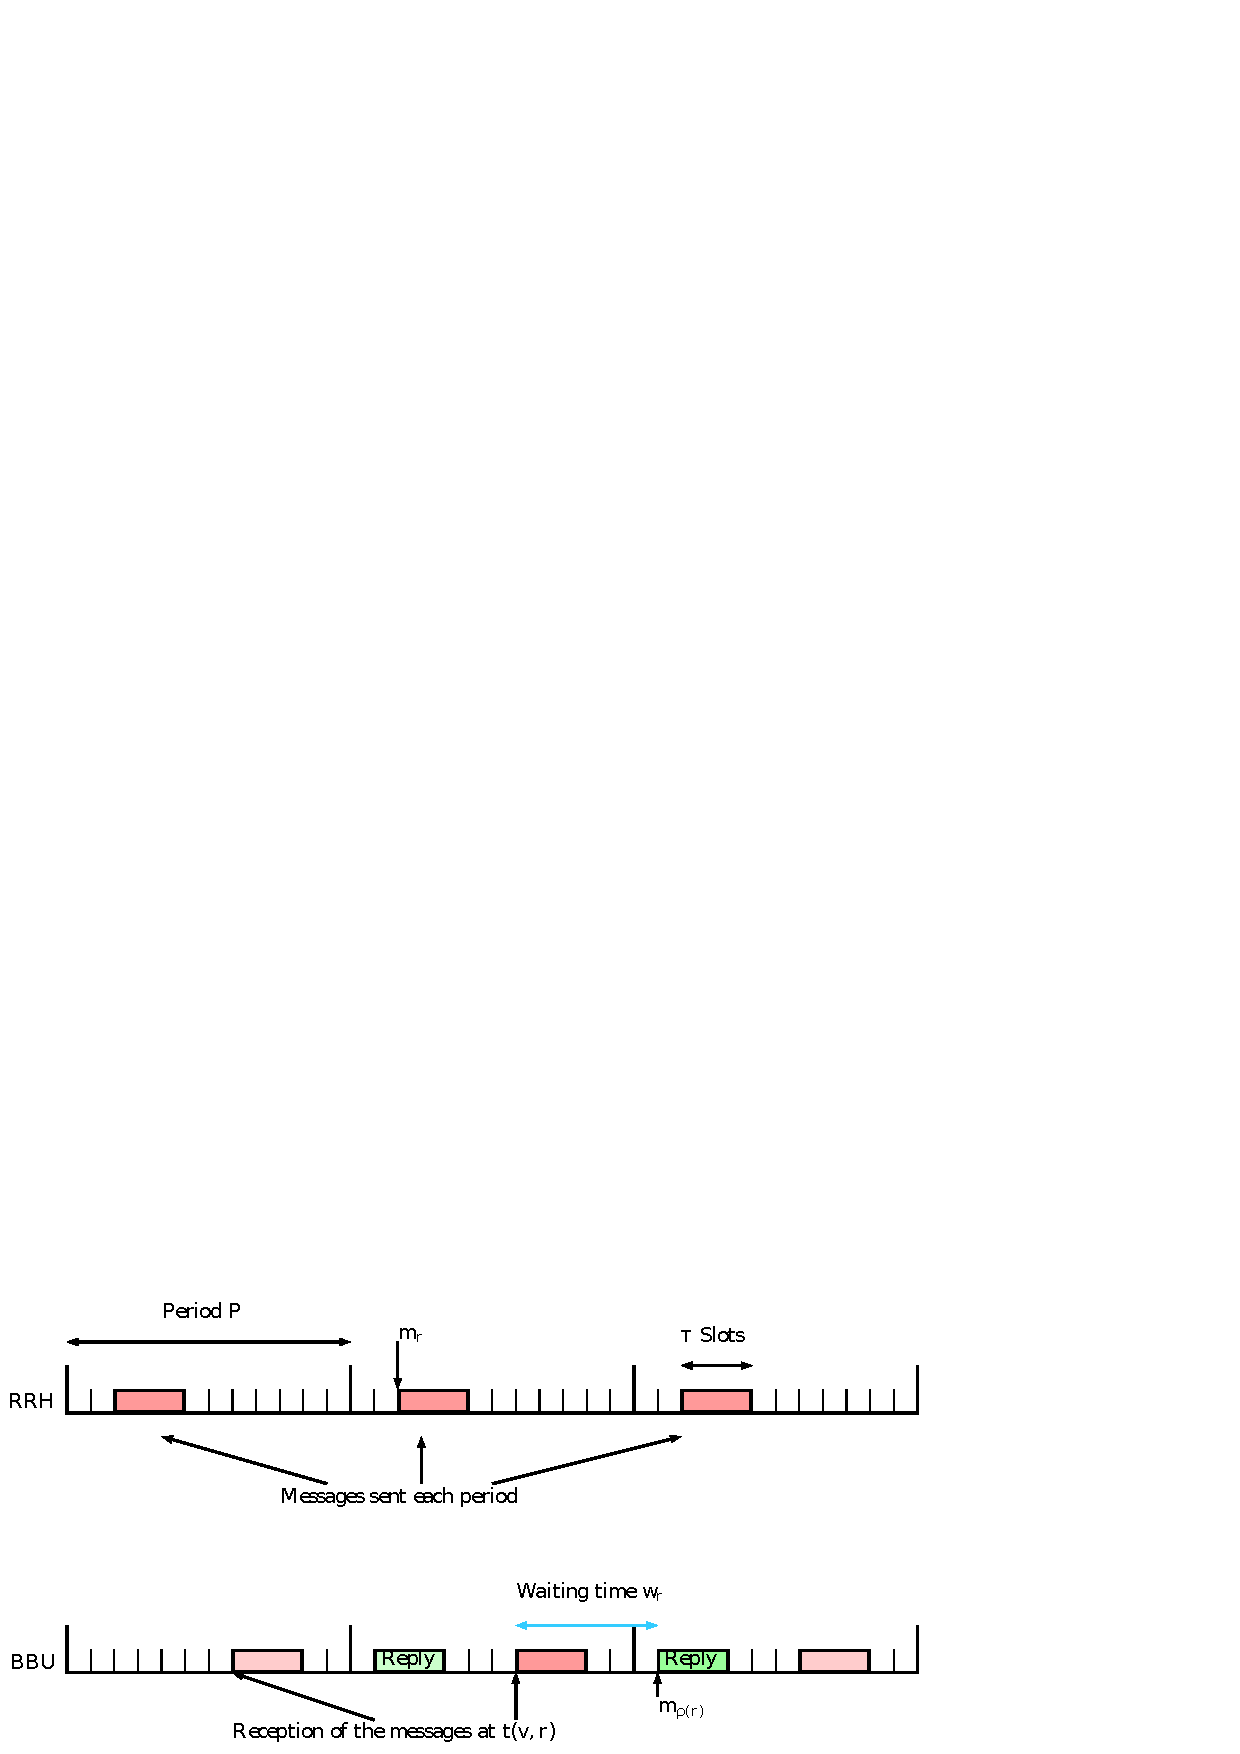
\includegraphics[width=0.90\textwidth]{rrh.pdf}
      \end{center}
      \caption{Periodic process}\label{fig:assignment}
      \end{figure}
      
      Note that, in the process we describe, we do not take into account the computation time a BBU needs to deal with one message. It can be encoded in the weight of the last arc leading to the BBU and thus we do not need to consider it explicitly in our model. 
      
      We define by {\bf jitter} of a frame the time at which the BBU receive the last datagram of the frame, minus the time at which the RRH has sent the first datagram of the frame, minus the length of the frame, minus the length of the route. In other words, if the RRH sends the datagram $d_0$ first on the route $r$ at time $m_r(d_0)$, and the BBU $v$ receive the last datagram of the frame $d_i$ at time $t(d_i,v,r)$, the jitter $J_r$ of a frame is then $J_r = t(d_i,v,r) - m_r(d_0) - \tau- \lambda(r)$.
      The whole process time for a route $r$ is equal to $PT(r)=\lambda(r)+ w_r+\lambda(r) + J_r$.      
      In the process time, we count the time between the time the first slot of the frame is emitted and the first time at which the first slot of the message comes back. Alternatively we could consider the time between the emission of the first slot and the reception of the last slot of the message, which adds $\tau$ to the process time. Both definitions are equivalent in our context where all messages are of size $\tau$, hence we chose the first definition which is slightly simpler. 
      Each route must respect a time limit that we call \emph{deadline}. To represent these deadlines, 
      we use a deadline function $d$, which maps to each route $r$ an integer such that $PT(r)$ must be less than $d(r)$.
      
%     The {\bf maximum process time} of the assignment $m$ of $(G,{\cal R})$ is defined by $MPT(m)=\max\limits_{r \in {\cal R}} PT(r)$.
      We consider the following decision problem.

      \noindent {\bf Periodic Assignment for Low Latency (\pall)} 

      \noindent {\bf Input:}  A symmetric routed network $(G,{\cal R})$, the integers $P$, $\tau$ and a deadline function $d$.
      
      \noindent {\bf Question:} does there exist a $(P,\tau)$-periodic assignment $m$ of $(G,{\cal R})$ such that for all $r \in {\cal R}$, $PT(r) \leq d(r)$?

      As a consequence of the $\NP$-hardness of \pra, we show in the next subsection that this problem is $\NP$-hard. 
      In Section~\ref{sec:PALL} we will study heuristics used to solve the search version of \pall (computing an assignment), also denoted by \pall for simplicity. In \pall, we have chosen to bound the process time of each route, in particular we can control the worst case latency. It is justified by our C-RAN application with hard constraint on the latency. It would be interesting to study the case of a constraint on the \emph{average} of process times (or equivalently waiting times) of routes, which may be more relevant in other contexts.

     
      The following table summarize the main notations used in the paper.
      \begin{center}
   \begin{tabularx}{0.5\textwidth}{|c|X|}
    \hline
     $(G,\cal R)$ & Routed network \\
     \hline
      $\Omega(u,v)$ & Weight of the arc $(u,v) \in A$ \\
      \hline
      $\lambda(u_i,r)$ & Latency of the vertex $u_i$ in $r$\\
         \hline
         $\lambda(r)$ & Length of the route $r$\\
         \hline
         $P$ & Period\\
         \hline
         $\tau$ & Size of a message\\
         \hline
         $ [t(v,r)]$& Set of time slots used by route $r$ at vertex $v$ in a period $P$\\
         \hline 
         $m=(m_0, \ldots ,m_{n-1})$& Assignment: an offset for each route\\
              \hline 
         $w_r$& Waiting time of the route $r$\\
            \hline 
         $PT(r)$& Process time of the route $r$\\
           \hline 
       $d(r)$ & Deadline of the route $r$\\
    \hline

      \end{tabularx}
      \end{center}

\bibliographystyle{ieeetr}
\bibliography{Sources}

\end{document}
